% Writeup for MDS
% David Lawrence Miller
% d.l.miller@bath.ac.uk
  
\documentclass[a4paper,10pt]{amsart}
 
% Load some packages
\usepackage{times, amsmath, amssymb, amsfonts, url, natbib, bm, rotating}
 
\usepackage{multirow}
\usepackage{graphicx}

% top matter
\title{Multidimensional scaling as a tool for smoothing over complex regions}
\author{David Lawrence Miller}
\email{d.l.miller@bath.ac.uk}
\address{Mathematical Sciences, University of Bath, Bath, United Kingdom}
 
% Shortcuts
% Probability
\newcommand{\prob}[1]{\mathbb{P}\left[ #1 \right]}
	% Hovitz-Thompson
\newcommand{\HT}{\hat{\tau}_{HT}}
% Schwarz-Christoffel
\newcommand{\sch}{Schwarz-Christoffel }
% fprime
\newcommand{\fprime}{f^\prime(z)}
% figure reference command
\newcommand{\fig}[1]{\emph{fig.} (\ref{#1})}
% Figure reference command
\newcommand{\Fig}[1]{\emph{Fig.} (\ref{#1})}
% equation reference command
\newcommand{\eqn}[1]{\emph{eqn.} (\ref{#1})}
% phi inverse
\newcommand{\phiinv}{\phi^{-1}}
% use other phi
\renewcommand{\phi}{\varphi}
%transpose
\newcommand{\tr}[1]{#1^{\text{T}}}
% diagonal
\newcommand{\diag}{\text{diag}}
% call \times \cross
\newcommand{\cross}{\times}


\begin{document}
 
% The abstract
\begin{abstract}
Here.
\end{abstract}
 
 
% New theorem for theorems
\newtheorem{thm}{Theorem}[section]
 
%New theorem for definitions
\newtheorem{defn}{Definition}[section]
 
\maketitle

%\markright{TECH. DETAILS OF SCHWARZ-CHRISTOFFEL MAPPING}

\section{Introduction}

Multidimensional scaling (MDS) or, as it is often referred to, principle coordinates (PCO) is a method commonly used in multivariate analysis to find a new configuration of points based on the distances between those points (\cite{chatfieldcollins}, p. 187.) In this new configuration, the Euclidean inter-point distances are approximately the same as their distances in the original data. Most often, MDS is used as a dimension reduction technique, finding a projection of data into lower dimensional space, while still retaining information about the distances between the points. It is closely related to other methods such as PCA (\cite{chatfieldcollins}, p. 200) and canonical correspondance analysis (\cite{terbraak}.)

Multidimensional scaling offers an obvious framework for the problem of smoothing over a region with a complex boundary. We can use the within-area distances to configure the points such that the distances between the points are (approximately) preserved.

\section{Multidimensional Scaling}

The basic concept behind MDS is to take the data, calculate their inter-point distances and then find a new coordinate system based on those inter-point distances. We do this by simply performing an eigen-decomposition on the matrix of distances between points.

\subsection{Finding the new point configuration}

We first define $d_{ij}$ as the distance between the points $i$ and $j$. These form a (symmetric) matrix, $D$, with $ij^{\text{th}}$ element $d_{ij}$. In our case, we would like $d_{ij}$ to be the shortest distance between the points, given the path between the points remains within the domain. How we find $d_{ij}$ is discussed in the next section, for the moment we assume that we know $d_{ij}$.

\cite{diaconis08} gives a clear definition of the algorithm (due to \cite{schoenberg35}) for finding the new locations of points given we know the $d_{ij}$s. 

First, take the unknown new locations and putting them in an $n \times p$ matrix, $X$. Let $S=X\tr{X}$; performing an eigen-decomposition we can see that $S=U\Lambda\tr{U}$. We may then represent $S$ in some arbitrary number of dimensions, $k$\footnote{We usually want $k<p$ to reduce the dimensionality of the problem.}, by picking the $k$ largest eigenvalues of $S$. In this case, we are interested in

\begin{equation}
\tilde{X}=\tilde{U}\tilde{\Lambda}^{1/2}.
\end{equation}

where a tilde indicates the $n \times k$ versions of $X$, $\Lambda$ and $U$.

We can relate $D$ to $S$ by first defining:

\begin{equation}
H = I-\frac{1}{n}\mathbf{1}\tr{\mathbf{1}}.
\end{equation}

By pre- and post-multiplying any matrix by $H$ we double centre it (row and column means are 0.) We then obtain\footnote{See \cite{diaconis08} for a simple proof.}:

\begin{equation}
S = -\frac{1}{2}HDH.
\end{equation}

So, in order to obtain a the new configuration of points using MDS (given that we have some set of inter-point distances) we merely need to double centre the matrix of distances and perform an eigen-decomposition.

Multidimensional scaling may be performed in \textsf{R} using the \texttt{cmdscale} function. 

\subsection{Inserting new points into the configuration}

It is likely that we may be in a position where the coordinate system has been found by MDS but we need to insert further points into our MDS representation; for example when further data is collected, or in order to predict over points not in the sample. In this case we would like to insert those new points into the configuration given by MDS\footnote{The insertion problem is also known as the ``out-of-sample problem'' (\cite{Trosset2008})}. A number of methods have been developed over the past 40 years. Two are covered here, first by \cite{gower1968} and then that of \cite{Trosset2008}.

\subsubsection{Gower's interpolation} 

Gower's method relies on taking a single new point $x_{\text{new}}$, and inserting at its distance from the original points ($\tilde{X}$) into a new dimension, orthogonal to $\tilde{X}$; the extra dimension is then projected on to the old axes. The technical details of the computation are detailed first, followed by some problems arising from the use of this method. 

We may find the new position, $\tilde{x}_{\text{new}}$, of some new datum $x_{\text{new}}$ using:

\begin{equation}
\tilde{x}_{\text{new}} = \frac{1}{2} \Lambda^{-1} \tr{\tilde{X}} \mathbf{d},
\label{gower}
\end{equation}

here $\Lambda$ ($k \cross k$) and $\tr{\tilde{X}}$ ($m \cross n$) are as above, $\mathbf{d}$ ($n \cross 1$) is defined as the distance between $x_{\text{new}}$ and the points in the original $\tilde{X}$. This formula (\ref{gower}) is commonly referred to as ``Gower's interpolation.''

Although the calculation is simple, it hides important pitfalls. 

\begin{enumerate}
\item If our sample ($\tilde{X}$) is not representative of the whole domain, the eigenvalues in $\Lambda$ are not the true eigenvalues; we may then insert the point incorrectly. This could happen if the sample is taken from only half of the space or, more pathologically, there were a trend in the sample locations, hence only a portion of the full information about the domain is included in the model. This would lead to the incorrect eigenvalues being calculated.

\item In the course of the projection onto the original MDS axes, we lose one of the coordinates (effectively truncating a dimension.) If the MDS axes were in two dimensions, it is possible that the point was not supposed to lie in the plane but rather this an extra dimension and its distance was truncated. This can cause distortions in the point configuration. An example of this is illustrated in \fig{bojinsert}. A more complete explanation and characterisation of this problem is given in \cite{Boj2009}. 

\item The above distortion is compounded when more than one point is added to the MDS configuration in an ``online'' sense. For example, say MDS has been performed on some set of points and then mapped them into the plane (giving $\tilde{X}$). Then suppose that new points are added into this configuration using Gower's interpolation. When the first point, $\tilde{x}_1$, is added say there is some error in its projection onto the plane from a third dimension, orthogonal to the first two. Adding in another point has the same problem, but now the $\tilde{x}_2$'s position is calculated with respect to $\tilde{x}_1$'s (potentially incorrect) position too. The third is then calculated using $\tilde{x}_1$ and $\tilde{x}_2$ and so on. This can be observed in \fig{gowererror}, where the red points should correspond to the gaps in the grid of black points, and the whole configuration should be identical to that of \fig{wt2dia} panel 2. 

\end{enumerate}

% diagram from Boj et al. 2009
\begin{figure}
\centering
% trim order l b r t
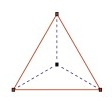
\includegraphics{figs/boj0.jpg} 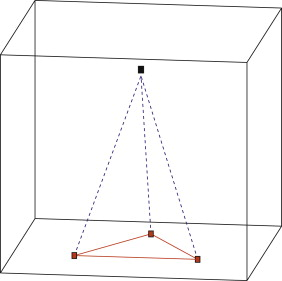
\includegraphics[width=1in]{figs/boj1.jpg} \\
\caption{Given the three points that make up the equilateral triangle in the left panel, if a new point is introduced then it will be mapped into a dimension orthogonal to that of the original points. This extra dimension is then truncated and the projection onto the plane used. Taken from \cite{Boj2009}.}
\label{bojinsert}
\end{figure}

Item (1) can be rectified by using an appropriately spaced grid on the domain to calculate the eigen-decomposition, thus ensuring that the whole area is covered. The sample points can then be inserted into this space.


The second and third points are linked, and combined lead us to believe that Gower's interpolation does not offer a solution to the insertion problem; we are both unable to insert points more than one at a time (thus making computation expensive) and, more importantly, are unable to insert points accurately without changing the representation space (\cite{Trosset2008}.)


\begin{figure}
\centering
% trim order l b r t
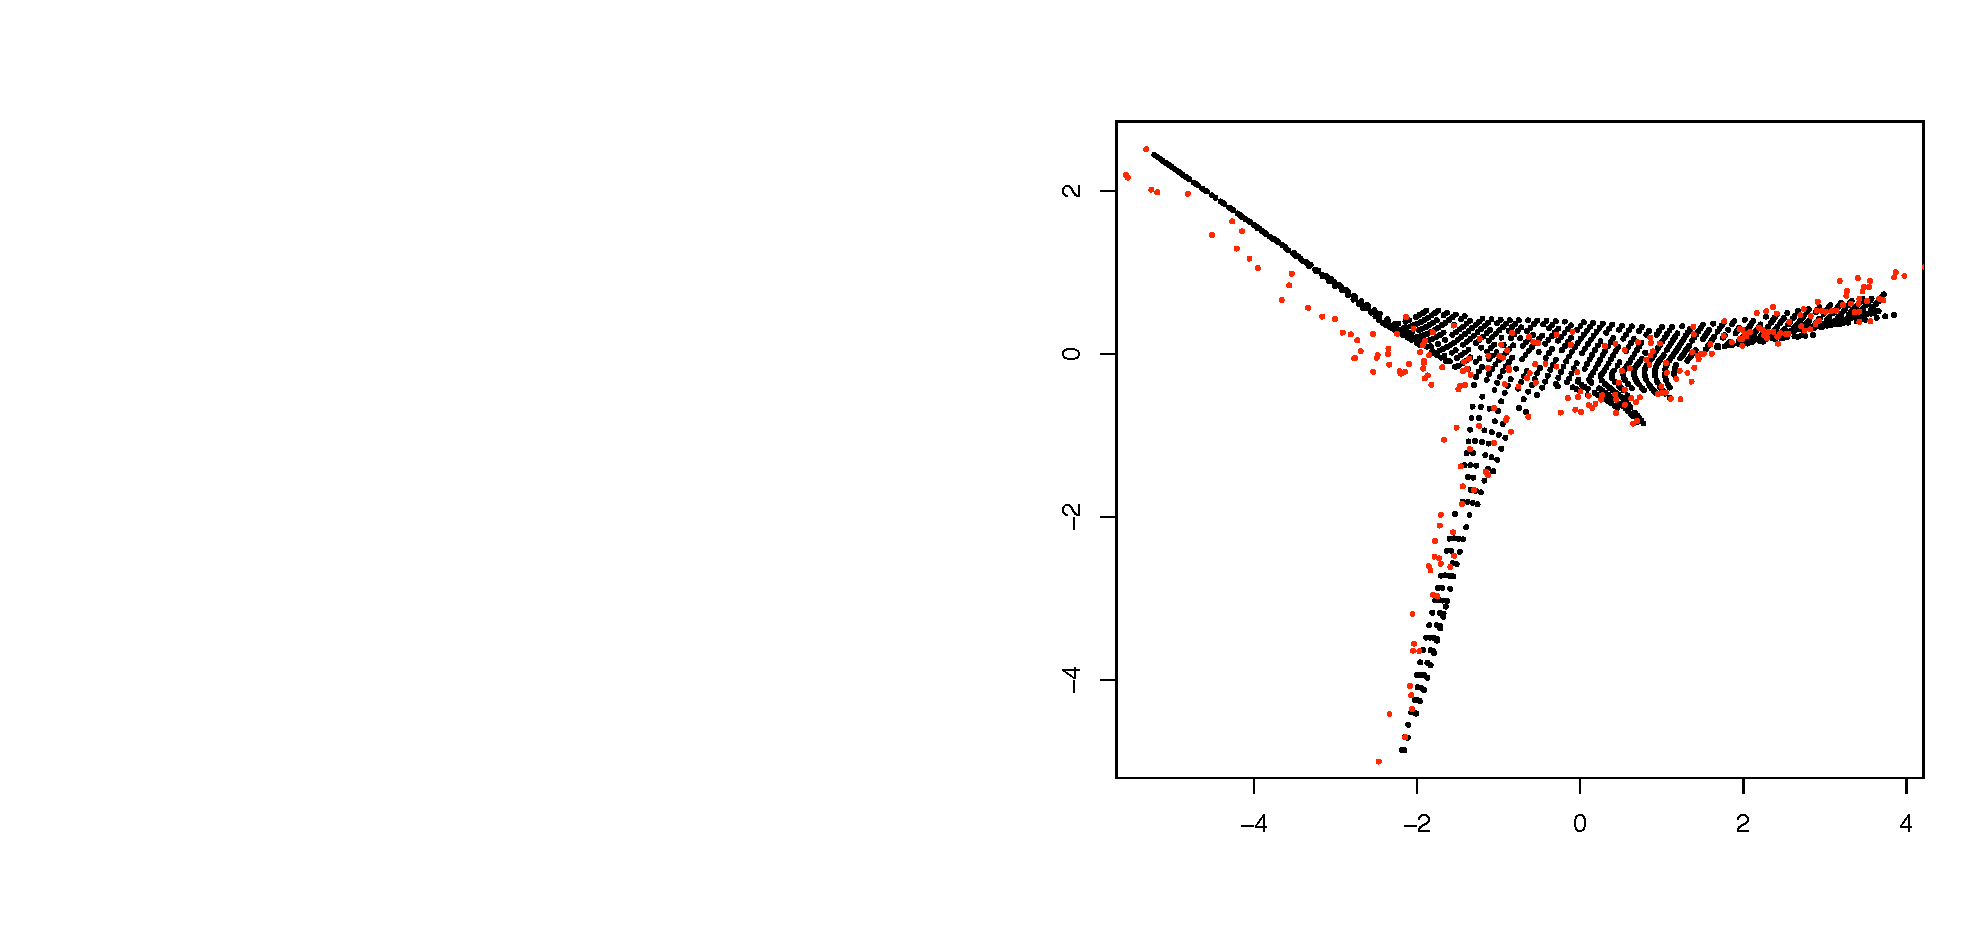
\includegraphics[width=4in]{figs/gowererror.pdf} \\
\caption{MDS configuration for the domain in \fig{wt2dia}. Black points are formed by the initial eigen-decomposition, where as the red points are positioned using Gower's interpolation from the initial MDS configuration. The red points should be positioned in the ``holes'' in the black grid.}
\label{gowererror}
\end{figure}


\subsection{Landmark MDS}



\subsection{The method of Trosset and Priebe}






\section{Finding the within-area distances}

The within-area distances to be fed to MDS are found using a novel algorithm. This works by tracing the inside sides of the polygon and then modifying the path by deleting and replacing portions of the path. 

Given that there is no direct path within the domain ($\Gamma$, say) between two points ($p_1$ and $p_2$, say), the algorithm proceeds as follows:

\begin{enumerate}
\item Draw a line between $p_1$ and $p_2$ (\fig{wdia}, ($i$)) and where they meet the boundary of $\Gamma$. Start the path as the lines from $p_1$, $p_2$ to their first intersection with the boundary of $\Gamma$. Then find the distance between these two intersection points in both directions, along the boundary (\fig{wdia}, ($ii$).) Choose the shorter of these add the paths between $p_1$, $p_2$ and the boundary and this is the starting path(\fig{wdia}, ($iii$).) 
\item Given a triple of vertices, ($v_i$, $v_{i+1}$, $v_{i+2}$) if the line between $v_i$ and $v_{i+2}$ is shorter than the path ($v_i$, $v_{i+1}$, $v_{i+2}$) and the line between $v_i$ and $v_{i+2}$ lies inside $\Gamma$ then delete $v_{i+1}$ (\fig{wdia}, ($iv$) and ($vi$).) This iterates over the entire path once, deleting all superfluous vertices. 
\item Given a triple of vertices, ($v_i$, $v_{i+1}$, $v_{i+2}$) if the path ($v_i$, some subset of the vertices of $\Gamma$, $v_{i+2}$) is shorter than the path ($v_i$, $v_{i+1}$, $v_{i+2}$) then replace $v_{i+1}$ with those elements of $\Gamma$ (\fig{wdia}, ($v$)). 
\item We then iterate between steps 2 and 3 until there has been no change from one run to the next (ie. convergence) or there have been too many iterations (\fig{wdia}, ($vi$).)
\end{enumerate}

% diagram for finding the shortest path in W
\begin{figure}
\centering
% trim order l b r t
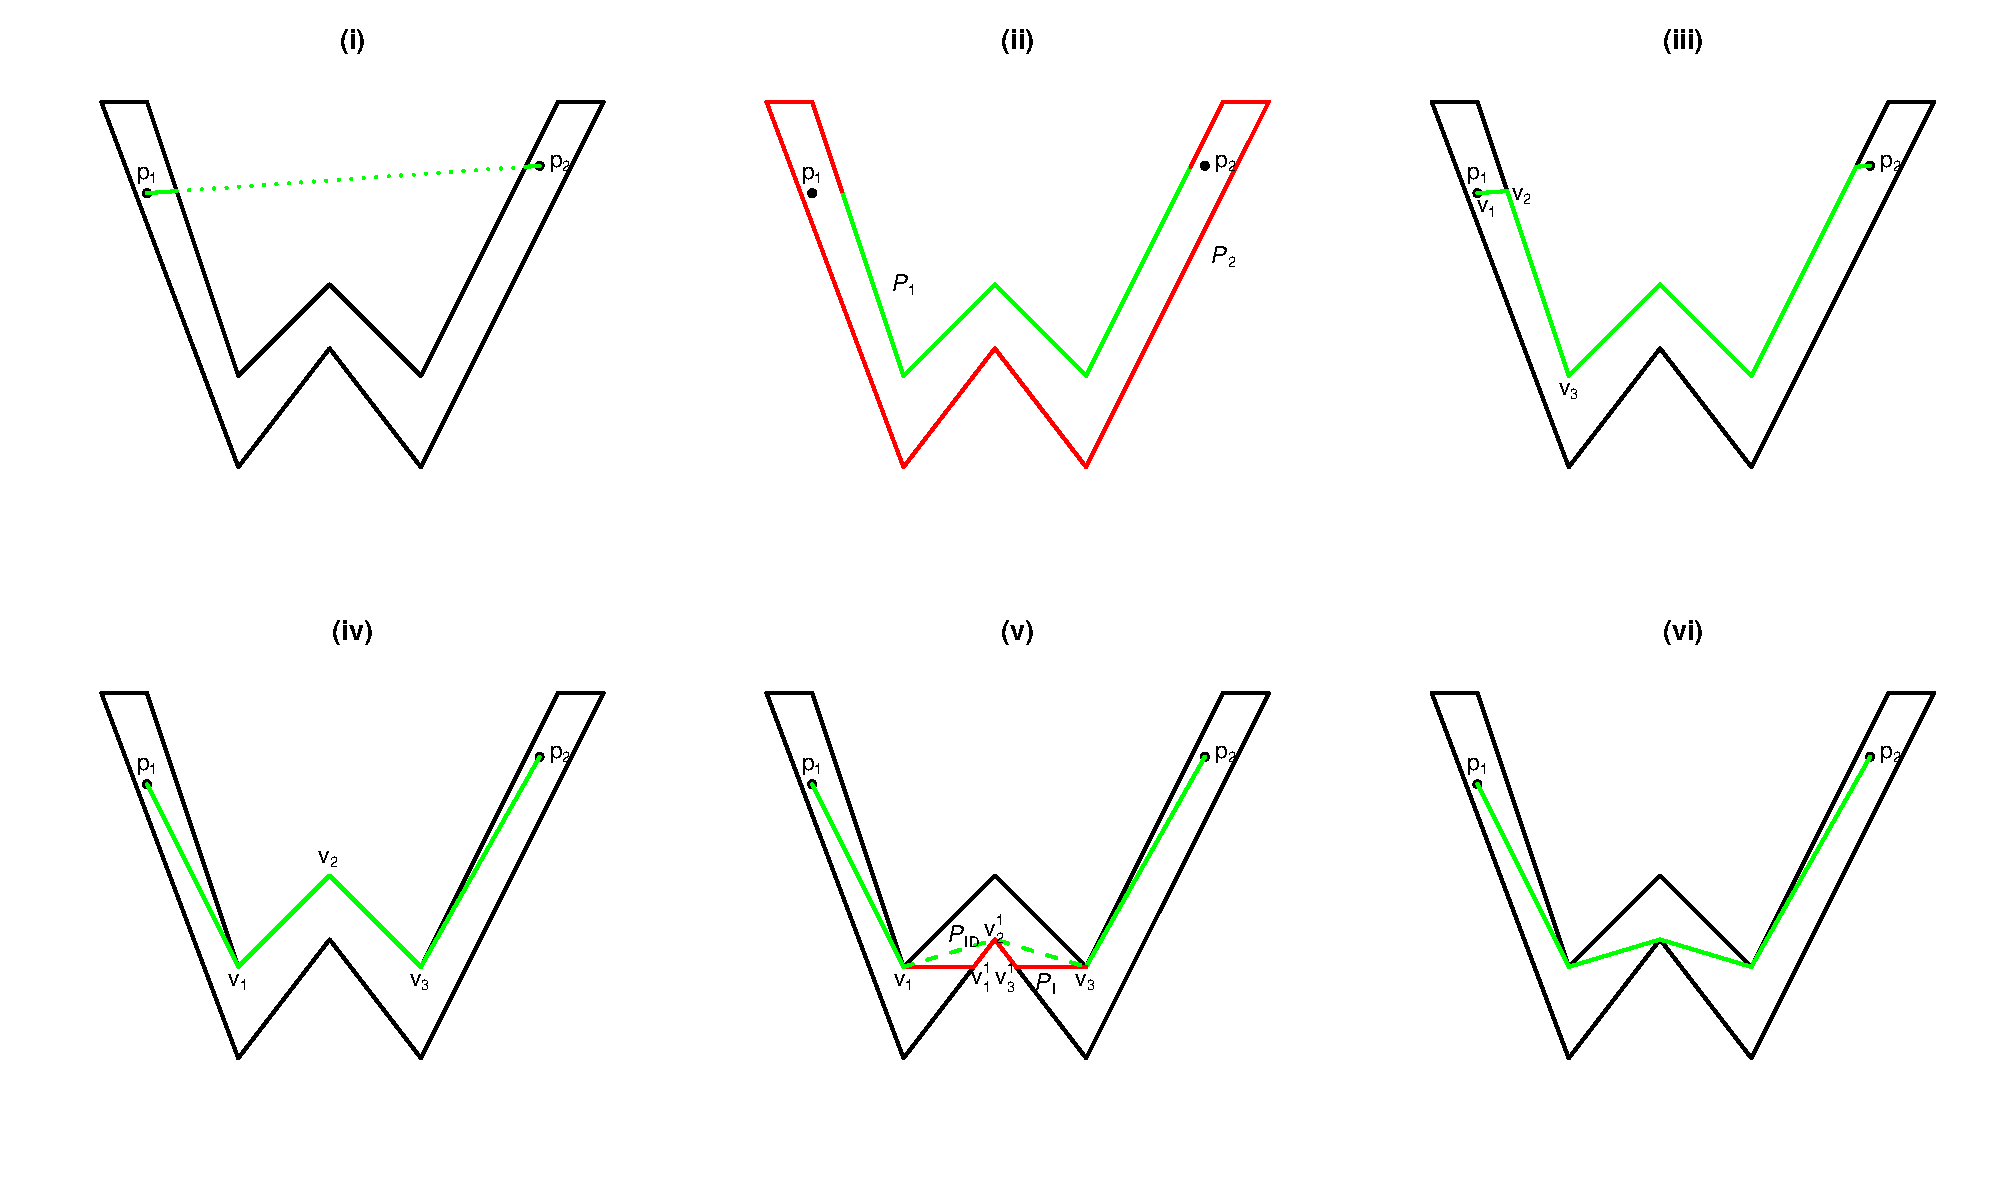
\includegraphics[trim=0in 0.5in 0in 0.25in, width=4in]{figs/wdia.pdf} \\
\caption{The green lines in ($i$) to ($vi$) show the path as the algorithm progresses from initial state to final, shortest path (bottom right.) }
\label{wdia}
% generate /phd-smoothing/mds-writeup/figs/distanceexplanation.R
\end{figure}



[[ euclidean distance analysis ]]


\section{Multidimensional scaling for complex domains}

Tying together the previous sections, we may now look at how, using MDS and our new algorithm, we can reconfigure the points in our domain.

\Fig{ramsay-mds} shows MDS being performed on the Ramsay horseshoe (\cite{ramsay}.) From this it is clear to see that performing MDS separates the two arms of the horseshoe.

% Ramsay MDSed 
\begin{figure}
\centering
% trim order l b r t
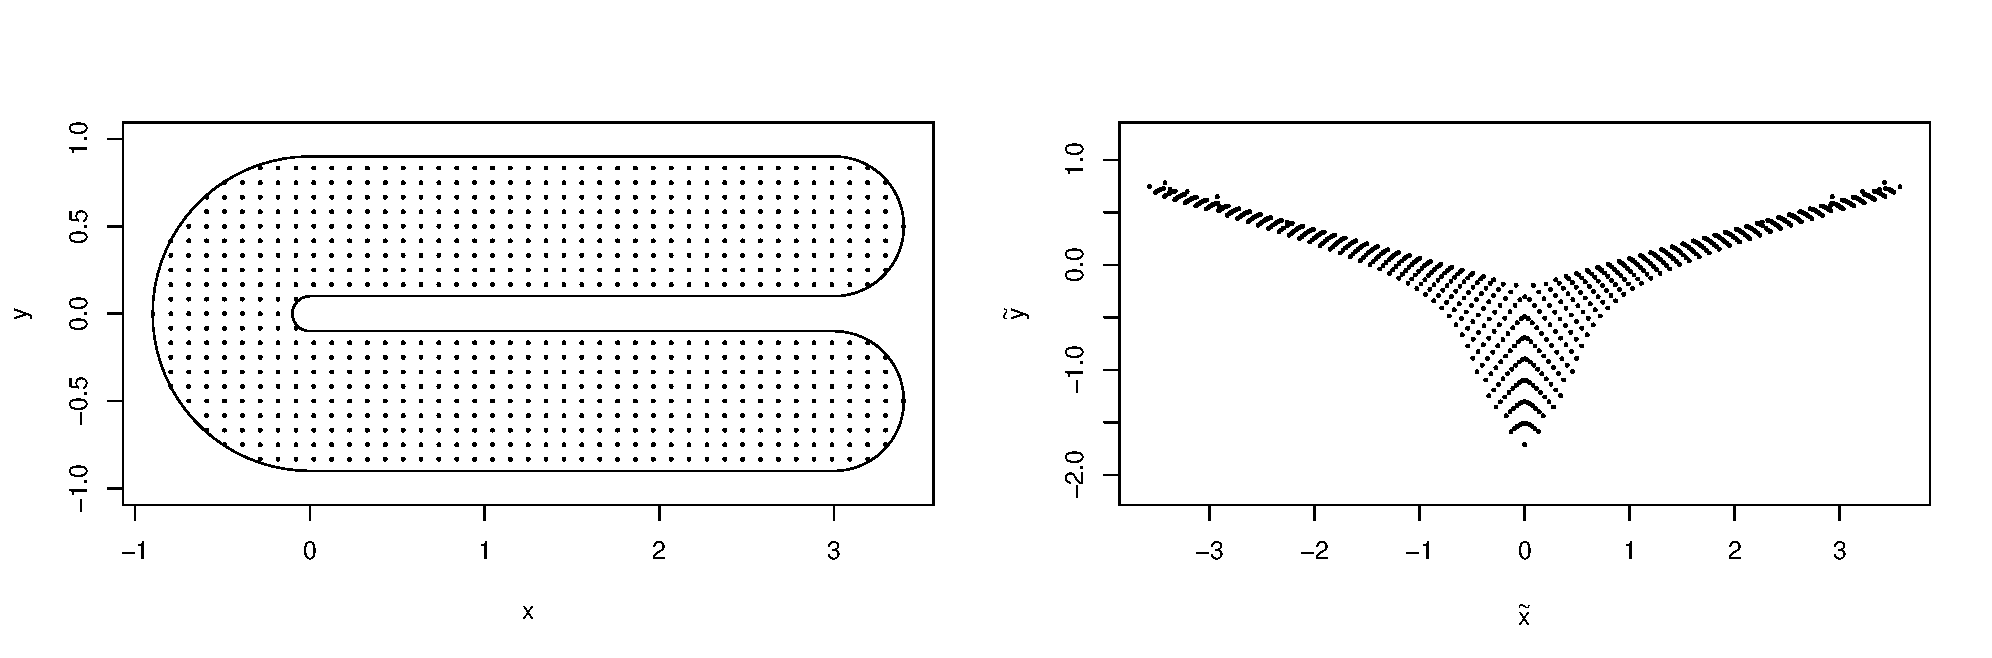
\includegraphics[trim=0in 0.5in 0in 0.25in, width=5.5in]{figs/ramsay-mds.pdf} \\
\caption{Left panel shows the horseshoe with 734 points. Right panel shows their configuration under MDS using the algorithm detailed above.}
\label{ramsay-mds}
% generate /phd-smoothing/mds-writeup/figs/ramsay-mds.R
\end{figure}

An advantage of the MDS approach is that in our eigen-decomposition we may pick an arbitrary number of eigenvectors to retain and push the original set of points into higher dimensions. Using three eigenvectors we get the configuration in \fig{ramsay-mds-3d}.

The two eigenvalues returned from running \texttt{cmdscale} in \textsf{R} when we ask for a 2-dimensional are 2615.5597 and 229.0039. Adding another dimension gives a third eigenvalue of 46.8754. Clearly significantly less variation is being explained in the third dimension, however this may well not be of primary concern if it prevents leakage.


\Fig{wt2dia} shows another domain which is more complicated than the horseshoe. The region has peninsulae which will cause similar problems to those found in the horseshoe. This domain is intended to replicate some of the problems that come about when dealing with coastlines.


An additional complication is that the peninsulae become smaller from left to right, thus the first couple of eigenvectors will be used to explain the variation along and across the bigger peninsulae.




% Ramsay MDSed 
\begin{figure}
\centering
% trim order l b r t
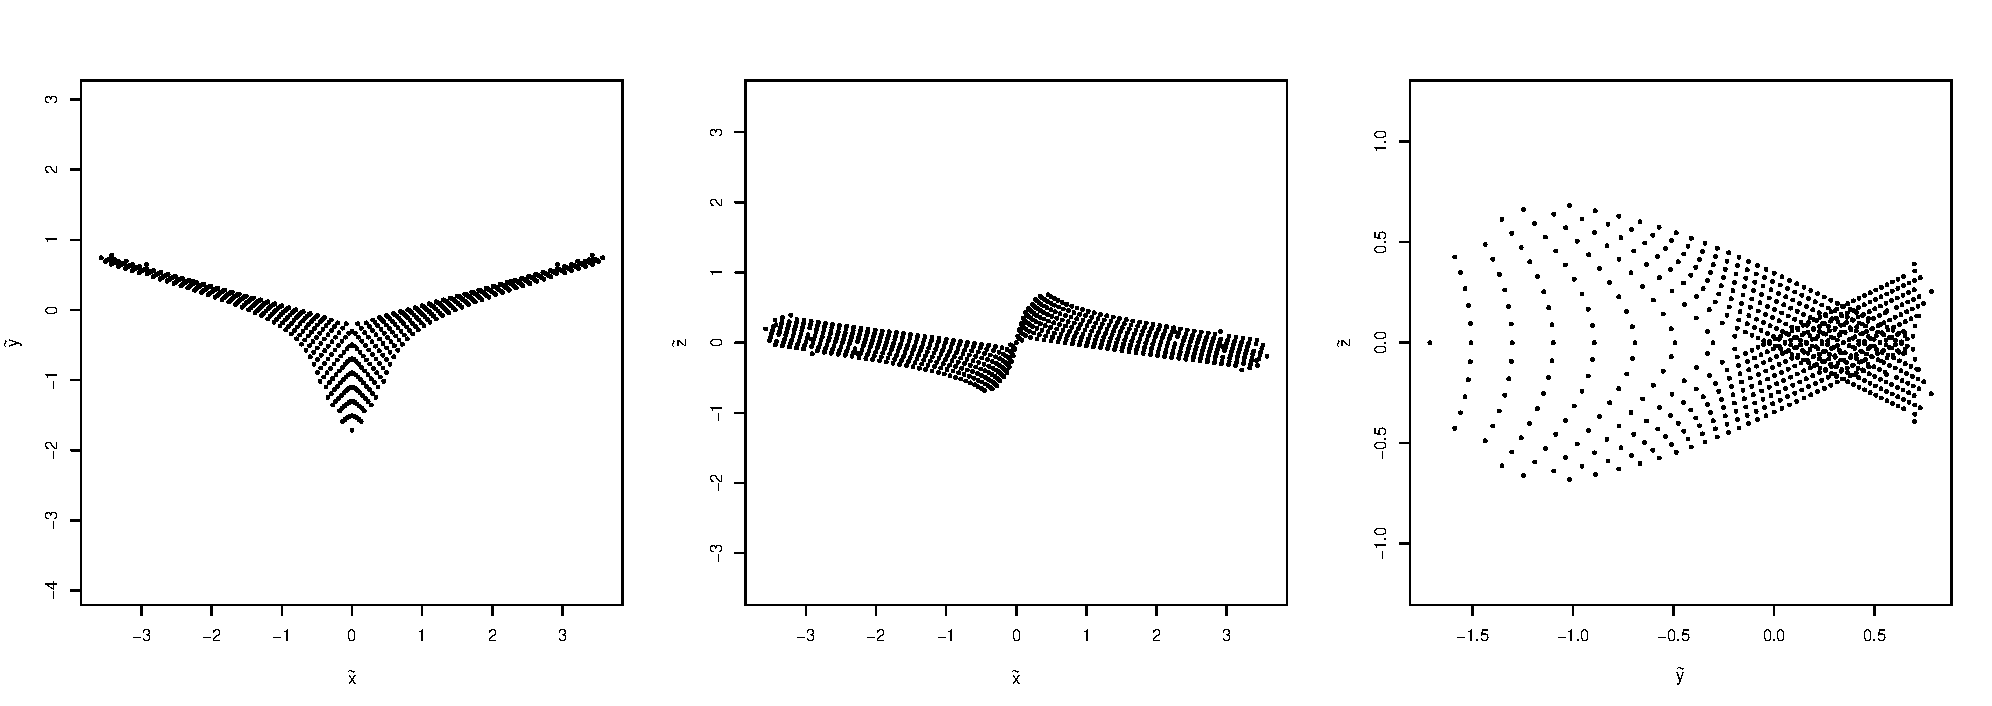
\includegraphics[trim=0in 0.5in 0in 0.25in, width=5.5in]{figs/ramsay-mds-3d.pdf} \\
\caption{Two-dimensional projections of the 3D mapping of the horseshoe.}
\label{ramsay-mds-3d}
% generate /phd-smoothing/mds-writeup/figs/ramsay-mds.R
\end{figure}

% plot of points in wt2.
\begin{figure}
\centering
% trim order l b r t
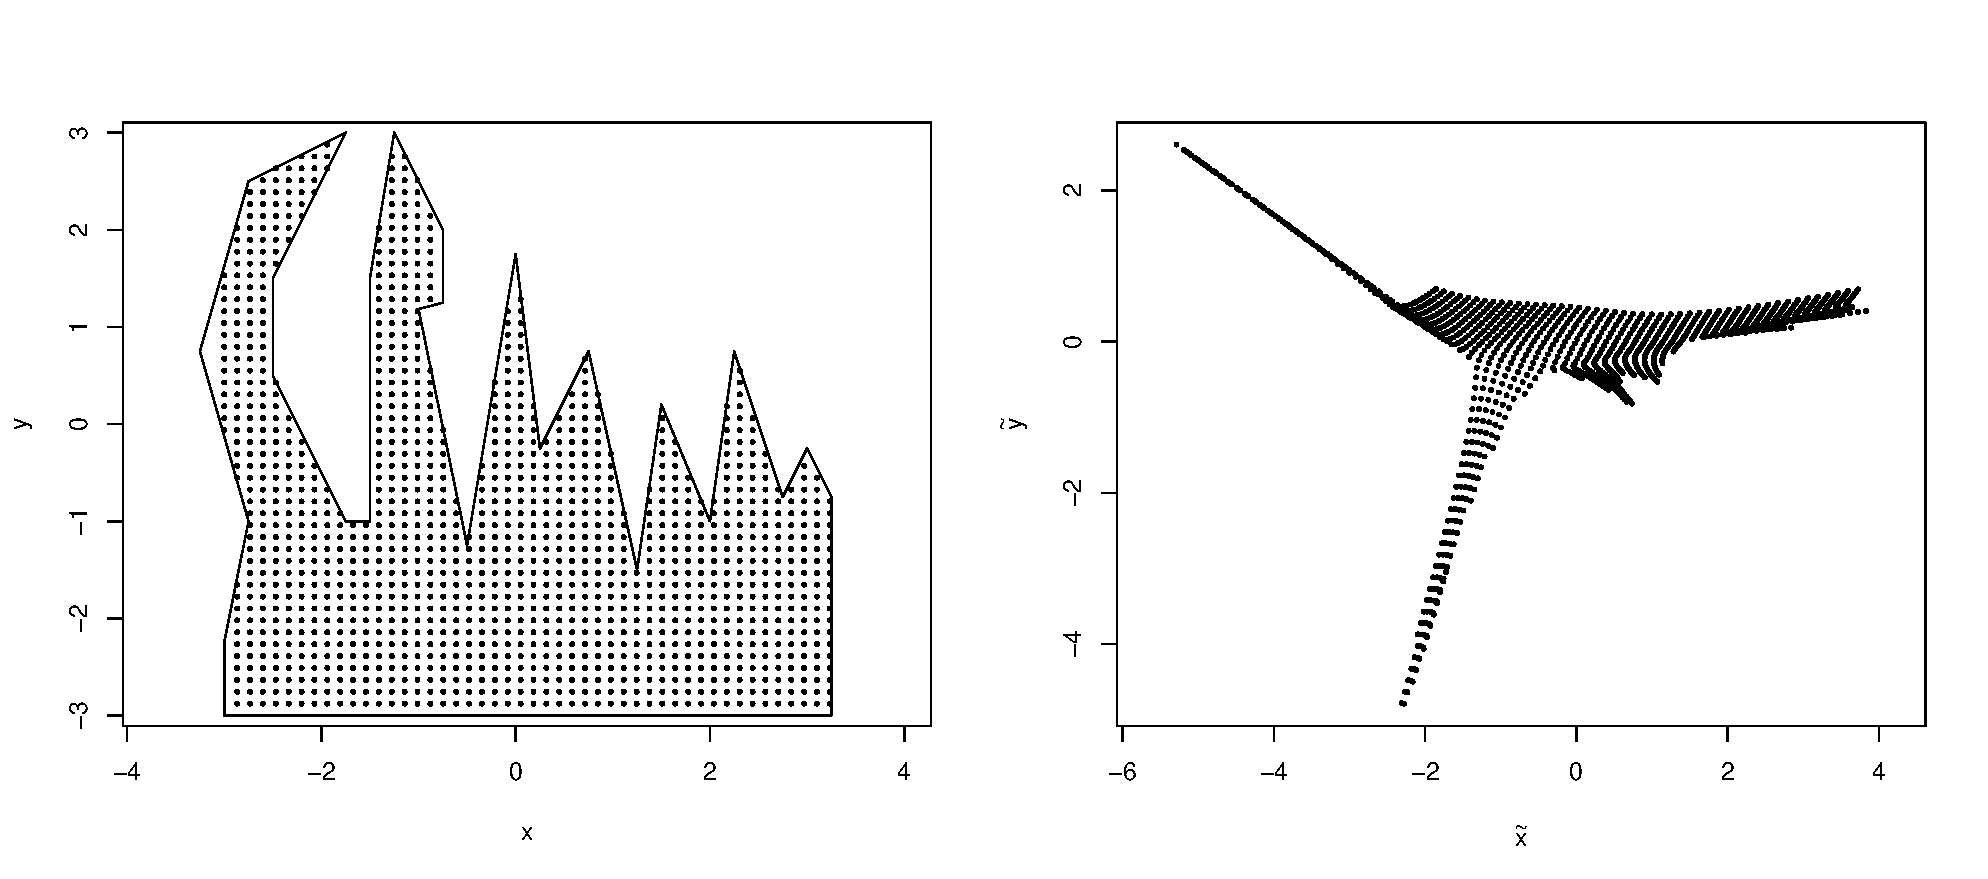
\includegraphics[width=6in]{figs/wt2-mds.pdf}\\
\caption{A domain with many peninsulae (left), and its MDS projection in two dimensions (right) for 1253 points in the domain.}
\label{wt2dia}
\end{figure}








\section{Simulation experiment}


VVVVV one run only

Ramsay
mds MSE= 0.002239077 
tprs MSE= 0.0651262 
soap MSE= 0.001455530 


wt2
mds=0.1291663
tprs=0.0760142
soap=0.02217734


3d sims

 summary(res.mse.mds)
   Min. 1st Qu.  Median    Mean 3rd Qu.    Max. 
0.04568 0.06914 0.08467 0.09712 0.10440 1.16000 
 summary(res.mse.tprs)
   Min. 1st Qu.  Median    Mean 3rd Qu.    Max. 
0.04369 0.06505 0.07444 0.07898 0.08667 0.28870 
 summary(res.mse.soap)
    Min.  1st Qu.   Median     Mean  3rd Qu.     Max. 
 0.01757  0.02123  0.02336  0.04722  0.02759 10.12000 





do plots of vis.gam() with too.far set low and overlay of points

boxplots



\section{Conclusions}


\bibliographystyle{plainnat}
\bibliography{mds-refs}

\end{document}
